% vim: spelllang=en_au
\documentclass[a4paper]{article}

\usepackage{geometry}
\usepackage{amsmath}
\usepackage{blkarray}
\usepackage{enumerate}
\usepackage{amssymb}
\usepackage{amsthm}
\usepackage{hyperref}
\usepackage{minted}
% \usepackage[symbol]{footmisc}
\usepackage{tikz}
\usetikzlibrary{automata}
\usetikzlibrary{positioning,arrows.meta,calc}
\usetikzlibrary{angles,intersections,quotes,arrows.meta}


\DeclareMathOperator{\lcm}{lcm}

\author{Kait Lam \\ \small \texttt{45294583} \\ \small {T02}}
\title{\textsc{Math3306} --- Assignment 2 (Submission)}
\date{6 September 2024}

\begin{document}

\maketitle


\section*{Question 1}
\subsection*{Question 1(a)}
\begin{center}
  \textit{Must a language over a single-letter alphabet be regular?}
\end{center}
% Of course not.
% Even with only a single letter, it is sufficiently powerful to represent any set of natural numbers.
% Define
% \begin{align*}
%   L = \{w \in \{\star\}^* ~|~ \ell(w) = \langle M, x \rangle \text{ and } \texttt{TM}_M\text{ halts on input }x\}.
% \end{align*}
% That is, the language of encoded pairs of Turing machine number and input, such that the Turing machine halts on the given
% input.
% This can be encoded as numerals in the usual way, i.e.\ by prime factors, then
% this is further encoded as unary within our single-letter alphabet.
% Were $L$ regular (that is, recognisable by a finite state automaton), this would easily decide the Halting problem,
% contradicting the known undecidability of this problem.
%
% Specifically, we could construct a TM which implements $\texttt{Halts}(m, x)$
% by encoding $\langle m, x  \rangle$ into unary, then emulating the FSA of $L$ and returning 1/0 depending on whether the unary word is accepted/rejected.
% As Turing machines are more powerful than FSA, this would be a straightforward task. 
% (An FSA can also be translated directly into a TM,
% e.g.\ like Q4(a) of Assignment 1).
%

% More generally, by way of encoding with prime factorisation and G\"odel numbering,
% any  can be represented as unary in a single-letter alphabet
% \hline
% Assume, with the intent of contradiction, that $L$ is regular.
% It may be irregular.
\noindent Consider the language
\begin{align*}
   L = \{ w \in \{\star\}^* ~|~ \ell(w)\text{ is prime}\}.
\end{align*}
Assume, with the intent of contradiction, that $L$ is regular and so the pumping lemma applies.
By pumping, there exists $p_L > 1$ such that for all $w \in L$, 
if $\ell(w) > p_L$, then there exists $x, y, z$ such that $w = xyz$ and 
\begin{enumerate}[(i)]
  \setlength{\itemsep}{0pt}
  \item $\ell(y) \ge 1$,
  \item $\ell(xy)  < p_L$, and
  \item $\forall n \ge 0, xy^nz \in L$.
\end{enumerate}
By the infinitude of primes, we can obtain
$w \in L$ such that $\ell(w) > p_L$.
Let $xyz=w$ be a decomposition as described.

First,
note that $\ell(xy) < p_L$ (property (ii)) specifies a fixed bound on the length of $xy$.
Therefore, since $w = xyz$, we can make $\ell(z)$ arbitrarily large by choosing a sufficiently large $w \in L$.
Without loss of generality, suppose we choose $w$ such that $\ell(z) \ge 2$.
% This will be useful later.

Now, by property (iii), we can construct a word with non-prime length and assert it must be in $L$.
To wit, the string
  $xy^{\ell(x)+\ell(z)}z$.
Observe,
\begin{align*}
  \ell(xy^{\ell(x)+\ell(z)}z) &= \ell(x) ~+~ \ell(y) (\ell(x) + \ell(z))~+~ \ell(z) \\
  &= (\ell(x) + \ell(z))\cdot(\ell(y) + 1)
\end{align*}
and note that (iii) provides that this word be within $L$.
%
To show that this factorisation demonstrates non-primality,
we should ensure both factors are greater than one.
For the right factor, note that $\ell(y) + 1 \ge 2$ by (i).
For the left factor, we have $\ell(x) + \ell(z) \ge 2$,
due to our earlier choice guaranteeing $\ell(z) \ge 2$.

Concluding,
$xy^{\ell(x)+\ell(z)}z$
is a word with non-prime length
(with factors $\ell(x) + \ell(z)$ and $\ell(y) + 1$).
The pumping lemma implies this word is in $L$ which contradicts
the original definition of $L$, so $L$ is a unary language which cannot be regular.

% As some technicalities,
% we note that due to infinitude of primes, we can obtain at least one $w \in L$ such that $\ell(w) > p_L$, in order to build our composite number.
%
%
% x + n y + z
% x + 
% (2x + 2z) (y + 1) = 2xy + 2x + 2zy + 2z

% x + z + (2x + 2z) * y = x + z + 2xy + 2zy

\subsection*{Question 1(b)}
\begin{center}
  \textit{Recognise $L = \{0^{2n}~|~ n \ge 0\}$ with a Turing machine.}
\end{center}
We will write a recursive algorithm:
\begin{enumerate}[(1)]
  \setlength{\itemsep}{0pt}
  \item If the string is empty, accept.
  \item Otherwise, divide the input unary number by two in this way:
    \begin{enumerate}
      \item move right and clear every second space until the end of the string, then
      \item move left and compress the string, collapsing all cleared spaces.
    \end{enumerate}
  \item Go to (1).
\end{enumerate}
The division algorithm implicitly ensures that the number is divisible by two, otherwise it will halt
due to missing transitions.
The full Turing machine is shown in Figure~\ref{fig:tm}.
For easier reading, we use the single symbol 1 instead of 0.
Be assured that these are exactly equivalent.

\begin{figure}[h]
  \begin{center}
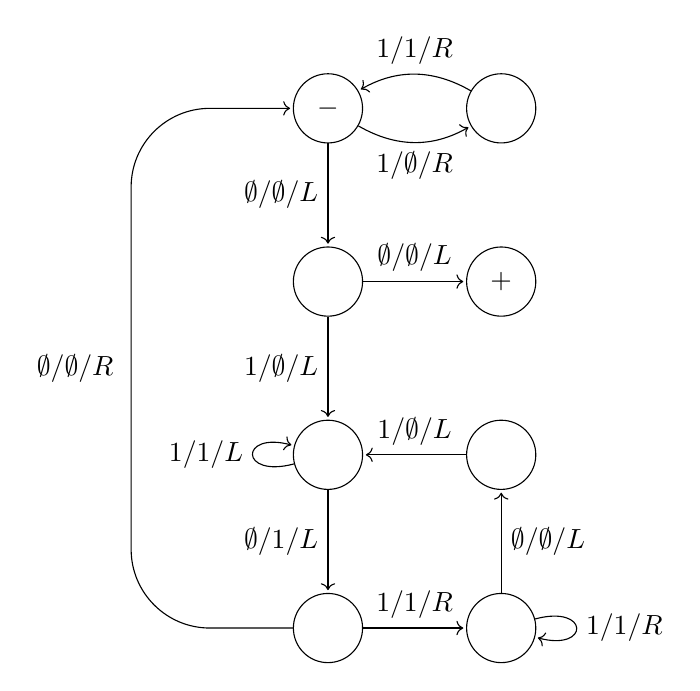
\begin{tikzpicture}[shorten >=1pt,node distance=2.2cm,on grid,auto] 

  \tikzset{
    rc/.style={rounded corners=2mm},
  }

   \node[state] (q0)   {$-$}; 
   \node[state] (first) [right=of q0] {};
   \path[->] (q0) edge [bend right] node [swap]{$1/\emptyset/R$} (first);
   % \node[state] (second) [right=of first] {};
   \path[->] (first) edge [bend right] node [swap]{$1/1/R$} (q0);

   \node[state] (base) [below=of q0] {};
   \path[->] (q0) edge node[swap] {$\emptyset/\emptyset/L$} (base);
   \node[state] (accept) [right=of base] {$+$};
   \path[->] (base) edge node {$\emptyset/\emptyset/L$} (accept);

   \node[state] (shift) [below=of base] {};
   \path[->] (base) edge node [swap]{$1/\emptyset/L$} (shift);
   \path[->] (shift) edge [loop left] node {$1/1/L$} (shift);

   \node[state] (shiftend) [below=of shift] {};
   \path[->] (shift) edge node [swap]{$\emptyset/1/L$} (shiftend);
   \node[state] (again) [right=of shiftend] {};
   \path[->] (shiftend) edge node {$1/1/R$} (again);
   \path[->] (again) edge [loop right] node {$1/1/R$} (again);
   \node[state] (restart) [above=of again] {};
   \path[->] (again) edge  node [swap]{$\emptyset/\emptyset/L$} (restart);
   \path[->] (restart) edge  node [swap]{$1/\emptyset/L$} (shift);

   \draw [->,rounded corners=1cm](shiftend) to
   ($(shiftend)+(-2.5, 0)$) to   node[xshift=-0.1cm]{$\emptyset/\emptyset/R$}($(q0)+(-2.5,0)$) to  (q0);
\end{tikzpicture}

  \end{center}
  \caption{A Turing machine.
     $\ominus$ and $\oplus$ denote the initial and accepting states, resp. 
  }\label{fig:tm}
\end{figure}

\section*{Question 2}
\begin{center}
  \textit{Is the language of (encoded) pairs of Turing machines with equivalent languages decidable?}
\end{center}
I think not.
If this language was decidable, it could be used to decide the halting problem.
We will demonstrate this.

Support $m$ and $x$ are given, encoding a Turing machine and an input under test.
We will compute $\texttt{Halts}(m, x)$.
First, transform $m$ into $m'$ such that
\begin{align*}
  T_{m'}(x') = \begin{cases}
    \textit{reject} &\text{if }x' \ne \text{$\star$}, \\
    \textit{accept} &\text{if }T_m(x)\text{ halts},\text{ and}\\
    \textit{undefined} & \text{otherwise}.
  \end{cases}
\end{align*}
Note that implementing $T_{m'}$ does \textit{not} require solving halting,
since we do not expect a concrete return value if $T_m(x)$ diverges.
$T_{m'}$ could be implemented from $T_m$ by %a simple check $x' = \text{``$\star$''}$, then
replacing all rejecting or missing edges
with an edge to an accepting state, 
then adding an initial check that $x' = \text{$\star$}$.
By careful construction,
the language of $T_{m'}$ is $\{\text{$\star$}\}$ if $T_m(x)$
halts and $\emptyset$ otherwise.



% Note we use $T_m$ and $T_{m'}$ to refer to the TMs encoded
% by $m$ and $m'$, respectively.


Suppose, with suspicion, that we now have a decider for $\texttt{EQ}_{\text{TM}}$.
We could then run the 
$\texttt{EQ}_{\text{TM}}$
decider and ask whether
$T_{m'}$ has the same language as the Turing machine recognising precisely $\{\star\}$.
By decidability, we have that the decider \textit{will} return either \texttt 1 or \texttt 0
for all inputs,
and this will represent whether the given TMs have the same language.
To implement our
$\texttt{Halts}(m, x)$,
we simply propagate the result of the decider.

This decides the undecidable halting problem, a contradiction, and so $\texttt{EQ}_{\text{TM}}$
cannot be decidable.



% (arbitrarily) it takes its input as binary strings.
% We construct 
% \begin{align*}
%   \texttt{Halts}(m, x) &= \texttt{EQ}_{\text{TM}}()
% \end{align*}



\section*{Question 3}
\begin{center}
  \textit{Show the following predicate is primitive-recursive.}
\end{center}
Given $f$ and $g$ primitive-recursive,
\begin{align*}
  p(x) &= \begin{cases}
    1 & \text{if } f(i) > g(j),\text{ for all } 1 \le i \le x \text{ and } 1 \le j \le x,\text{ or } \\
    0 & \text{otherwise.}
  \end{cases}
\end{align*}
This can be expressed using bounded minimisation
(in this case, acting like bounded iteration).
\begin{align*}
  p(x) := \big(~x+1 = \mu(1\le i \le x).~(x+1 \ne \mu(1\le j \le x).~f(i) \le g(j))~\big)
\end{align*}
The desired predicate returns 1 iff $f(i)$ is always
greater-than $g(j)$ within
the square $1 \le i,j \le x$.
We implement this by searching within this region for counter-examples,
using bounded minimisation.
The bounded minimisation operator returns the least index satisfying its
argument function, if it exists, otherwise it returns one more than its upper bound.

We check the result of the inner $\mu$ to see if we have found \textit{any} counter-example,
and at the outer $\mu$, we check the inverse to ensure there have been \textit{no} counterexamples.
This will make sure we return the correct result of the predicate.
We assume the equality and disequality operators return either 0 or 1.

(Essentially, this encodes
\begin{align*}
  p(x) &= \neg \exists(1 \le i \le x).~\exists(1 \le j \le x).~f(i) \le g(j) \\
       &= \forall(1 \le i \le x).~\forall(1 \le j \le x).~f(i) > g(j),
\end{align*}
since ``$x + 1 \ne \mu(\cdot).~P$'' implements ``$\exists(\cdot).~P$''.)

\section*{Question 4}
\begin{center}
  \textit{
  Prove SOL  is {NP}-complete (both {NP}-hard and itself in {NP}).}
\end{center}
First we prove that SOL  is {NP}-hard by reducing 3SAT to SOL.
For simplicity, we use the symbols T and F (loosely corresponding to true and false) instead of the colours red and blue.

A 3SAT formula with $c$ clauses is to be translated into a
$(c+6)\times(c+6)$ SOL board.
This is computable in a polynomial amount of time, since the contents
of each board cell can be determined in polynomial time.
We introduce the following correspondences
from 3SAT concepts into SOL:
\begin{itemize}
  \setlength{\itemsep}{0pt}
  \item atoms\footnote{an atom is a variable or a negated variable.} are encoded as columns, one column each for its regular and negated forms
    (so, 6 columns for 3SAT), and
  \item a disjunctive clause is encoded as a row,
    with a T in columns corresponding to atoms appearing in the clause and empty elsewhere.
\end{itemize}
The semantics of 3SAT are mapped in this way:
\begin{itemize}
  \setlength{\itemsep}{0pt}
  \item Validity of the
    disjunction is enforced by each row containing at least one stone,
    corresponding to at least one true atom within the clause. 
  \item The conjunction of clauses is caused by each clause appearing in its own line, as 
    the rules of SOL require every row to be non-empty (and so every clause must be satisfied).
  \item The law of excluded middle\footnote{actually, the law of non-contradiction.} is implemented by a special $2\times2$
    square at the bottom of each pair of $x$ and $\neg x$ columns (explained more below).
    This leverages the rule requiring 
    each column hold stones of at most one colour. 
  \item A winning position is interpreted as a result of ``sat'' and an unwinnable
    position is ``unsat''.
\end{itemize}

\subsection*{Further details}
For each variable, the $x$ and $\neg x$ columns are  related
through a $2 \times 2$ control square, shown below.
This pattern ensures that a T symbol appears in at most one of the two columns.
\begin{align*}
\begin{blockarray}{cc}
x & \neg x  \\ \hline
\begin{block}{cc}
  \vdots & \vdots  \\
  \text F & \text F  \\
  \text T & \text T  \\
\end{block}
\end{blockarray}
\end{align*}
Consider the square in isolation: how could this pattern be won?
Each column may only hold one symbol, so either T or F needs to be cleared
from one column, and the other symbol from the other.
The result must be one column with F and one with T, forcing the 
cells above the F column to be cleared of T.
Further, there are no other cells in these two rows, so
the player may not clear both symbols in the same row.
The F/T in this control square can be thought of as that atom's valuation.

In the rest of the playing field, however,
the player may clear T symbols even if the atom column has a valuation of T.
The presence of a T symbol indicates both that the corresponding
atom is true \textit{and} that it is relevant for the solution.
One symbol in each row is enough to satisfy SOL, just like
one true atom satisfies the disjunction.

Finally, we note that this can be simplified by omitting the T row of the $2 \times 2$ control square. This allows a winning configuration to have both F symbols still present. In such cases, both columns must be cleared of T and the formula is
satisfiable regardless of the value of that variable.

It can be further simplified by using only one column per variable (3 columns total) and using T for $x$ and F for $\neg x$.
This requires preprocessing to eliminate trivially-satisfied clauses but
avoids the need for a LEM-enforcing square.
We do not use this because we enjoy logic puzzles.

\subsection*{Example}
Consider the 3SAT problem of
\begin{align*}
  (x \vee \neg x \vee z) \wedge (\neg x \vee y \vee z).
\end{align*}
This would be translated as the $8\times8$ game board below. 
The two columns further to the right are entirely blank.
Note the column labels are informational only and not part of the game.
\begin{align*}
\begin{blockarray}{cccccc}
  x & \neg x&
  y & \neg y&
z & \neg z
\\ \hline
\begin{block}{cccccc}
  \text T & \text T & & & \text T \\
          &\text T  & \text T & & \text T \\
  \text F & \text F  \\
  \text T & \text T  \\
          && \text F & \text F  \\
          && \text T & \text T  \\
          &&&& \text F & \text F  \\
          &&&& \text T & \text T  \\
\end{block}
\end{blockarray}
\end{align*}
This board has a winning configuration, such as the one below.
The SAT solution can be read off from the control blocks.
Here, it is $x = y = z = \textit{False}$.
\begin{align*}
\begin{blockarray}{cccccc}
  x & \neg x&
  y & \neg y&
z & \neg z
\\ \hline
\begin{block}{cccccc}
  & \text T & & & \\
          &\text T  & & & \\
  \text F & \\
  & \text T  \\
          && \text F & \\
          && & \text T  \\
          &&&& \text F & \\
          &&&& & \text T  \\
\end{block}
\end{blockarray}
\end{align*}

\subsection*{Proof of reduction}
We argue that this mapping is sound and complete.
\begin{itemize}
  \item For completeness (satisfiable 3SAT $\longrightarrow$ winnable SOL configuration),
    take the satisfying 3SAT valuation and the corresponding
    initial game board.
    For each atom column, if it holds, clear all F from the column, and if it doesn't, clear all T from the column.
    The result is a winning configuration.

    Uniqueness of column colour is since each column had one colour cleared,
    and non-emptiness of row is since each clause is satisfied and by structure
    of the control squares.

  \item For soundness
    (unsatisfiable 3SAT problem $\longrightarrow$ no winning SOL board),
    we prove the contrapositive:
    if a SOL board constructed from a 3SAT problem is winnable, then 
    the 3SAT problem is satisfiable. 
    Suppose we have a winning game board.
    Read off the variable valuations from the control squares,
    as per the example.

    By uniqueness of column colour and the control squares, we have 
    that for all each variable, $x$ and $\neg x$ have opposite values.
    Since we constructed one row per clause and 
    we have at least one stone per row,
    we know every disjunctive clause has at least one true atom,
    satisfying the proposition.

\end{itemize}
We conclude the 3SAT problem is faithfully reducible to SOL.
Since 3SAT is NP-hard, this demonstrates SOL is NP-hard.

\subsection*{Proof of NP}
We show SOL is in NP by constructing a polynomial-time verification algorithm
for the game of SOL.

We take as input the initial $n\times n$ SOL board and the final
$n \times n$ board state,
and we need to determine if the final board is a winning configuration. Note
that this information is polynomial (approx.\ $2n^2$ in size).

First, check that the final state is a subset of the initial board,
i.e.\ the player has not cheated by adding new stones.
This is about $n^2$ operations.
Then, check both the column rule (uniqueness within a column)
and the row rule (non-emptiness within a row).
These will be $n^2$ each.

If all these checks pass, the solution is validated.
Otherwise, it is rejected.
This polynomial-time checking algorithm shows that SOL is in NP. 







\end{document}

